\documentclass[12pt]{article}

\usepackage{amsmath}
\usepackage{comment}
\usepackage{amscd}
\usepackage[utf8]{inputenc}
\usepackage{fancyhdr}

\usepackage{calc}
\usepackage{natbib}
\usepackage[american]{babel}

\setlength{\paperheight}{11in}
\setlength{\paperwidth}{8.5in}
\addtolength{\voffset}{-1.0in}
\addtolength{\hoffset}{-1.0in}
\setlength{\topmargin}{1in}
\setlength{\oddsidemargin}{1in}
\setlength{\evensidemargin}{1in}
\setlength{\textwidth}{\paperwidth - 2in}
\setlength{\textheight}{\paperheight - 2in}
\setlength{\footskip}{36pt}
\setlength{\marginparsep}{0.5cm}
\setlength{\marginparwidth}{1.5cm}
\setlength{\headheight}{0pt}
\setlength{\headsep}{0pt}



\pagestyle{fancy}
\renewcommand{\headrulewidth}{0pt}
\lhead{}
\chead{}
\rhead{}
\lfoot{}
\cfoot{\thepage}
\rfoot{}



\usepackage{Sweave}
\begin{document}


\begin{center}
  {\LARGE An rbrothers tutorial}\\\ \\
  {Jan Irvahn and Vladimir N. Minin \\ 
    Department of Statistics, University of Washington Seattle, WA, 98195, USA
  }
\end{center}

This is a tutorial demonstrating the usage of the java program, DualBrothers, in R.  To get started, install the rbrothers R package from R-forge. 
\begin{verbatim}
> install.packages("rbrothers", repos="http://R-Forge.R-project.org")
\end{verbatim}
The rJava package and a couple of other packages will need to be installed.

Start R and load the rbrothers library.
\begin{Schunk}
\begin{Sinput}
> library(rbrothers)
\end{Sinput}
\end{Schunk}

Copy the KAL153.phy file from the rbrothers package to your current working directory.
\begin{Schunk}
\begin{Sinput}
> my.align = read.dna(file=system.file("extdata/KAL153/KAL153.phy", 
 	  	   package="rbrothers"))
> write.dna(my.align,"KAL153.phy")
\end{Sinput}
\end{Schunk}

Now you can run DualBrothers with a single command.
\begin{Schunk}
\begin{Sinput}
> db<-dualbrothers(123,"KAL153",format="interleaved")
\end{Sinput}
\end{Schunk}

If you already have the output files of a DualBrothers run you can read the information in directly.
\begin{Schunk}
\begin{Sinput}
> db<-readdb("KAL153")
\end{Sinput}
\end{Schunk}

Plots can be created with the following commands.

\begin{Schunk}
\begin{Sinput}
> plot(db,threshold=.5)
\end{Sinput}
\end{Schunk}
\begin{Schunk}
\begin{Sinput}
> plottree.db(db,type="phylogram",threshold=.5)
\end{Sinput}
\end{Schunk}



\begin{figure}[!t]
  \centering
\includegraphics{rbrothers_tutorial-dbfigure1}
\caption{The top plot shows site specific posterior probabilities for the two most probable phylogenetic tree topologies. The bottom plot shows the site specific posterior probability of a breakpoint.}
\label{KALplot}
\end{figure}  

\begin{figure}[!t]
  \centering
\includegraphics{rbrothers_tutorial-dbfigure2}
\caption{These are the two most probable phylogenetic tree topologies.}
\label{KALplot2}
\end{figure}  


The average number of breakpoints, the posterior probability of at least one breakpoint and DualBrothers parameters associated with the run can be easily accessed.
\begin{Schunk}
\begin{Sinput}
> summary(db)
\end{Sinput}
\begin{Soutput}
DualBrothers output for KAL153 
4 sequences of length 8588 

MCMC settings: 
length of the MCMC chain: 2100000 
burn-in length: 100000 
subsample frequency: 200 

Prior parameters: 
prior mean number of substitution process change points: 5 
prior mean number of topology change points: 0.693 

average number of breakpoints in the posterior: 2.1 
The posterior probability of at least one breakpoint was 1  (> 0.999  required for a Bayes factor > 1000). 
3 trees considered 
\end{Soutput}
\end{Schunk}

You can calculate a 95\% Bayesian credible interval for the first breakpoint.
\begin{Schunk}
\begin{Sinput}
> breakpointCI(db,1000,3000)
\end{Sinput}
\begin{Soutput}
The 95% credible interval for a single break point between nucleotide number 1000 and nucleotide number 3000 is:
 2.5% 97.5% 
 1666  1985 
\end{Soutput}
\end{Schunk}


%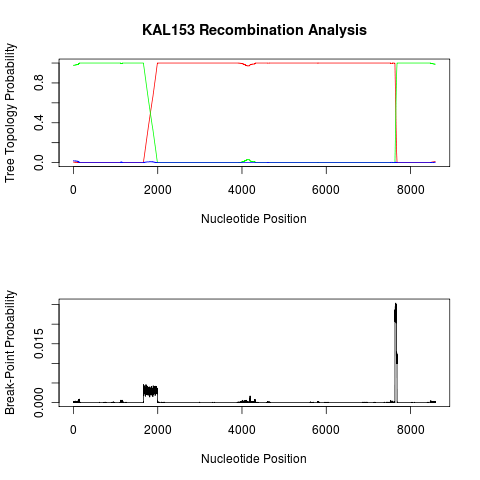
\includegraphics[width=70mm]{KAL153plot1.png}
%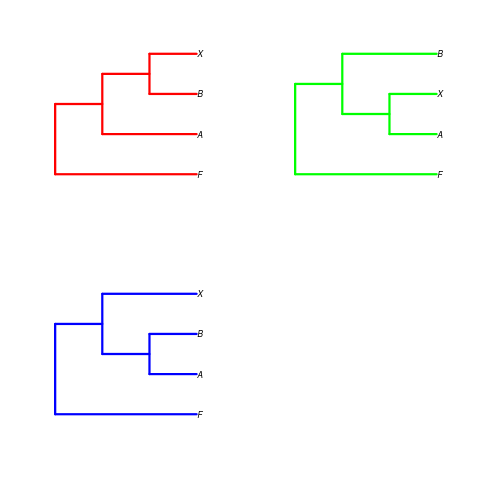
\includegraphics[width=70mm]{KAL153plot2.png}


\end{document}

